% !TEX encoding = UTF-8 Unicode

\documentclass[a4paper]{article}

\usepackage{color}
\usepackage{url}
\usepackage[T2A]{fontenc} % enable Cyrillic fonts
\usepackage[utf8]{inputenc} % make weird characters work
\usepackage{graphicx}
\usepackage{array}

\usepackage[english,serbian]{babel}
%\usepackage[english,serbianc]{babel} %ukljuciti babel sa ovim opcijama, umesto gornjim, ukoliko se koristi cirilica

\usepackage[unicode]{hyperref}
\hypersetup{colorlinks,citecolor=green,filecolor=green,linkcolor=blue,urlcolor=blue}

%\newtheorem{primer}{Пример}[section] %ćirilični primer
\newtheorem{primer}{Primer}[section]

\begin{document}

\title{Analogni računari\\ \small{Seminarski rad u okviru kursa\\Tehničko i naučno pisanje\\ Matematički fakultet}}

\author{Aleksandar Končalović, Uroš Janković, Veljko Strugar, Veljko Josipović\\ kontakt email adresa autora}
\date{2.~novembar 2022.}
\maketitle

\abstract{
U ovom tekstu je ukratko prikazana osnovna forma seminarskog rada. Obratite pažnju da je pored ove .pdf datoteke, u prilogu i odgovarajuća .tex datoteka, kao i .bib datoteka korišćena za generisanje literature. Na prvoj strani seminarskog rada su naslov, apstrakt i sadržaj, i to sve mora da stane na prvu stranu! Kako bi Vaš seminarski zadovoljio standarde i očekivanja, koristite uputstva i materijale sa predavanja na temu pisanja seminarskih radova. Ovo je samo šablon koji se odnosi na fizički izgled seminarskog rada (šablon koji \emph{morate} da ispoštujete!) kao i par tehničkih pomoćnih uputstava. 

\tableofcontents

\newpage

\section{Uvod}
\label{sec:uvod}
Pre nastanka prvih digitalnih računara, za izračunavanja su se koristili \textbf{analogni računari}. Najstariji primer takvog računara je takozvani Mehanizam sa Antikitere za koji se veruje da datira iz drugog veka pre nove ere. \cite{antikitera}\\
Računari tog doba su se koristili za predviđanje raznih dešavanja u stvarnom svetu poput pomračenja Sunca i Meseca, tačnog vremena plime i oseke, a kasnije i u naučne i ratne svrhe.\\
Čak i nakon nastanka prvih digitalnih računara, analogni su jedno vreme bili smatrani moćnijim i bržim.

\section{Princip rada analognih računara}
Analogni računari vrše izračunavanja tako sto obrađuju kontinualne veličine. Iako se  za njihov rad najčešće koristi električna struja i napon, to nije nikakvo pravilo, i bilo koja kontinualna veličina može da se upotrebi. Te veličine su na primer: \begin{itemize}
				\item Količina vode u cevima
				\item Zategnutost opruga
				\item Intenzitet magnetne sile
				\item Vibracije tla kod seizmografa
				\item Visina vode kod mašine za predvidjanje plime i oseke \cite{tide}
				\item Položaj zubčanika
				\item Položaj čekrka
				\item Temperatura raznih supstanci
			\end{itemize}
			
\bigskip

    \begin{primer}
    Uzmimo kao primer operaciju sabiranja dva borja koristeći količinu vode u posudama.\\
    Da bismo sabrali dva broja, recimo 3 i 5, poterebno je da imamo tri identične čaše sa skalom za merenje nivoa vode u čaši. Sabiranje možemo izvrsiti prateći sledeći postupak:\begin{enumerate}
        \item U prvu čašu nalijemo vode do trećeg podeoka (za broj 3).
        \item U drugu čašu nalijemo vodu do petog podeoka (za broj 5).
        \item Prelijemo sadržaj obe čaše u treću času koju smo ostavili praznu.
        \item Očitamo visinu vode tako što gledamo do kog podeoka je stigla.
        \item Uočavanjem da je visina vode stigla do osmog podeoka (za broj 8) dobili smo rezultat sabiranja.
    \end{enumerate}
    \end{primer}
    
\bigskip

    \begin{primer}
    Za množenje dva broja možemo koristiti električnu struju, napon i otpor.\\
    Da bismo pomnožili dva broja, recimo 3 i 5, poterebno je da imamo voltmetar i električno kolo koje se sastoji od strujnog generatora i promenljivog otpornika. Množenje možemo izvrsiti prateći sledeći postupak:\begin{enumerate}
        \item Podesimo strujni generator tako da generiše električnu struju od tri ampera (za broj 3).
        \item Podesimo promenljivi otpornik tako da mu otpor bude pet oma (za broj 5).
        \item Postavimo pipalice voltmetra na krajeve otpornika.
        \item Očitamo napon na voltmetru.
        \item Uočavanjem da je napon očitan na volmetru jednak petnaest volti (za broj 15) dobili smo rezultat množenja.
    \end{enumerate}
    \centering Ovaj postupak koristi formulu
    \centering $$ U = R*I $$\\
    \centering za računanje proizvoda.
    \end{primer}


\section{Hidrointegrator Mike Alasa}	
\label{sec:hidrointegrator}

Hidrointegrator Mihaila Petrovića Alasa je prva analogna računska mašina koja radi na principu kretanja tečnosti. Petrovićev rad na ovom uređaju najavio je još 1896. profesor mehanike na Velikoj školi u Beogradu Ljubomir Klerić.\\
Usavršena verzija, koja se smatra završnim rešenjem hidrointegratora, opisana je u američkom časopisu za matematiku (eng.~{\em American Journal of Mathematics}) 1899. godine.\cite{hidrointegrator}\\
Na slici \ref{fig:h1} prikazana je skica hidrointegratora. 

\bigskip

\begin{figure}[h!]
\begin{center}
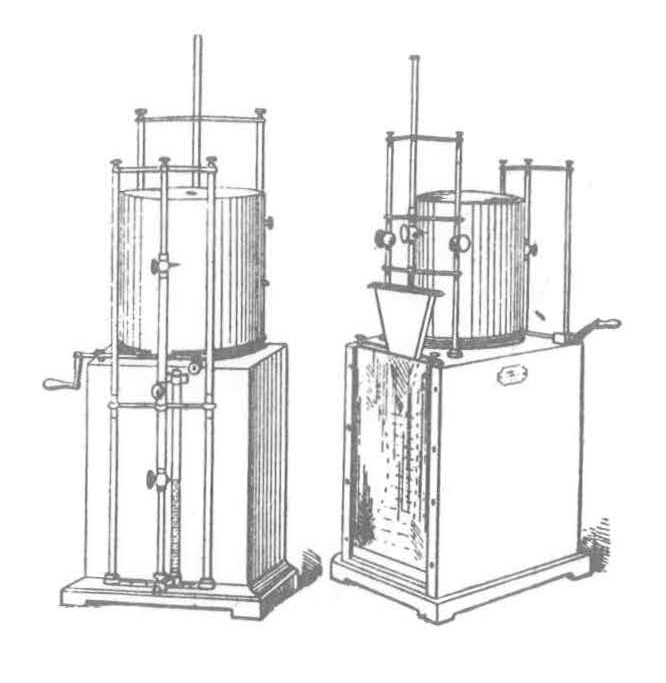
\includegraphics[scale=1.5]{h1.jpg}
\end{center}
\caption{Petrovićeva skica hidrointegratora. }
\label{fig:h1}
\end{figure}

\bigskip





\section{Slike i tabele}
\label{slike_i_tabele}

Slike i tabele treba da budu u svom okruženju, sa odgovarajućim naslovima, obeležene labelom da koje omogućava referenciranje. 

\begin{primer} Ovako se ubacuje slika. Obratiti pažnju da je dodato i 
\begin{verbatim}
\usepackage{graphicx}
\end{verbatim}

\begin{figure}[h!]
\begin{center}
\includegraphics[scale=0.75]{pande.jpg}
\end{center}
\caption{Pande}
\label{fig:pande}
\end{figure}

Na svaku sliku neophodno je referisati se negde u tekstu. Na primer, na slici \ref{fig:pande} prikazane su pande. 
\end{primer}

\begin{primer} I tabele treba da budu u svom okruženju, i na njih je neophodno referisati se u tekstu. Na primer, u tabeli \ref{tab:tabela1} su prikazana različita poravnanja u tabelama.

\begin{table}[h!]
\begin{center}
\caption{Razlčita poravnanja u okviru iste tabele ne treba koristiti jer su nepregledna.}
\begin{tabular}{|c|l|r|} \hline
centralno poravnanje& levo poravnanje& desno poravnanje\\ \hline
a &b&c\\ \hline
d &e&f\\ \hline
\end{tabular}
\label{tab:tabela1}
\end{center}
\end{table}

\end{primer}





\section{Primeri analognih racunara}
\label{sec:naslov1}


U ovom poglavlju cemo navesti primere raznih analognih racunara. 


\subsection{Logaritmar}
\label{subsec:podnaslov1}

Logaritmar je jedan od najosnovnijih analognih racunara koji je kreiran u ranom 17. veku od strane William Oughtreda. U pocetku se koristio za mnozenje i deljenje, a nesto kasnije se pokazalo da je primenjliv za izracunavanja eksponencijalnih, logaritamskih i trigonometrijskih funkcija takodje.

Sastoji se od dve letvice istih duzina od kojih sira ima u sebi usecen zleb po kojem klizi uza letvica. Povrh sire letvice takodje po zlebu klizi providna plocica na kojoj je ucrtana tanka linija koja sluzi za iscitavanje rezultata. Na obe letvice je upisano vise redova brojeva koji slizu za racunanje.
Racunanje se sprovodi pomeranjem uze letvice duz sire, pri cemu se nad zadatim brojevima vrse razne operacije.
Navodno, prva posada koja je sletela na povrsinu meseca, predvodjena Nilom Armstrongom, ponela je sa sobom razne elektronske sprave, ukljucujuci i logaritmar.

\subsection{Al-Jazarijev sat u zamku}
\label{subsec:podnaslov2}

Al-Jazarijev sat je starinski sat, visok skoro 3.5 metra, koji je koristio neke od slozenih koncepata masinstva za svoj rad. Osim prikazivanja vremena, bio je u mogucnosti da obavlja i druge funkcije kao sto je prikazivanje solarnih i lunarnih orbita. Kreiran od strane Ismail al-Jazaria, sat u zamku, jedan je od najvecih izuma svih vremena. Sagradjen je tokom prve decenije 13. veka. 

\subsection{Diferencijalni analizator}
\label{subsec:podnaslov3}

 Diferencijalni analizator su izmislila dva inzenjera, Vannevar Bush i Harold Hazen, tokom ranih 1930-ih. Dizajniran je za resavanje slozenih diferencijalnih jednacina. Ova tehnologija koristi mehanicke aranzmane za obradu podataka i izracunavanje resenja.

\subsection{Analogni termometar}
\label{subsec:podnaslov4}

Analogni termometar koristi stepenastu skalu i svojstva zive da bi ispunio svoj rad. Ziva, koje je tecna na sobnoj temperaturi, pri zagrevanju se siri. Time se omogucava potrosacu da dijagnostikuje bolesno stanje tela. Temperatura tela je analogni signal. Stoga je termometar koji meri telesnu temperaturu odlican primer analognih racunara. 

\subsection{Brzinomer}
\label{subsec:podnaslov5}

Brzinomer je uredjaj koji detektuje brzinu vozila u pokretu, uglavnom u kilometrima po casu. Brzina se pokazuje pomocu igle kojoj je dozvoljeno da se slobodno krece u skladu sa analognim signalom koji prima. Kabl brzinomera je na jednom kraju pricvrscen za osovinu zubcanika, a na drugom kraju za trajni magnet. Ovaj magnet je povezan sa metalnom casom za brzinu bez fizicke veze izmedju njih. Casa za brzinu je povezana indikatorom pomocu induktorske sipke na kojoj je pricvrscena opruga. Vrteca spoljna osovina menjaca rotira magnet. Magnetno polje koje generise pokretni magnet privlaci metalnu casu brzine. Ovo mehanicko kretanje casice za brzinu se koristi za skretanje igle. Ovaj otklon igle ukacuje na brzinu vozila.


\subsection{Analogni sat}
\label{subsec:podnaslov6}


Iako su digitalni satovi sve cesce u upotrebi, tradicionalni, analogni satovi idalje obavljaju posao u mnogim domacinstvima. Mnogi od nas nisu ni svesni da je analogni sat oblik analognog racunara. On koristi kristal kvarca koji je podlozan piezoelektricnom efektu. Napon koji obezbedjuje baterija, analogni signal, omogucava piezoelektricnom kristalu da vibrira brzinom od tacno 32 768 vibracija u sekundi. Uz pomoc ovih vibracija, generise se impuls, a jedan impuls je vremenski ekvivalentan jednoj sekundi. Dakle, jedna sekunda je jednaka 32 768 vibracija piezoelektricnog kristala.


\section{n-ti naslov}
\label{sec:naslovN}

Ovde pišem tekst. 
Ovde pišem tekst. 
Ovde pišem tekst. 
Ovde pišem tekst. 
Ovde pišem tekst. 

\subsection{... podnaslov}
\label{subsec:podnaslovK}

Ovde pišem tekst. 
Ovde pišem tekst. 
Ovde pišem tekst. 
Ovde pišem tekst. 
Ovde pišem tekst. 

\subsection{... podnaslov}
\label{subsec:podnaslovM}

Ovde pišem tekst. 
Ovde pišem tekst. 
Ovde pišem tekst. 
Ovde pišem tekst. 
Ovde pišem tekst. 

\section{Elektronski analogni rčunari}
		\label{sec:naslov4}
		
		\par Mane mehaničkih analognih računara kao što su:
		\begin{itemize}
			\item njihova veličina i veoma zahtevno održavanje
			\item brzina izračunavanja ograničena momentom inercije komponenata
			\item limitirana preciznost na svega nekoliko procenata usled mrtvog hoda
			\item dug vremenski interval potreban za podešavanje računara za specifične probleme jer je blio potrebno izvršiti veliki broj prespajanja
		\end{itemize}
		bile su samo neki od razlog za kratak životni vek mehaničkih analognih računara i rađanja ideje o \emph{elektronskim analognim računarima} koji su brzo postali veoma uticajani.
		\par Prvi elektronski analogni rčunar implementirao je nemački naučnik Helmut Helcer (nem. Helmut Hölzer) sredinom Drugog svetskog rata tokom svog rada na kontroli letenja namenskog dalekometnog artiljerijskog oružja za strategijsko bombardovanje što je zahtevalo ogroman broj izračunavanja. \cite{Holzer}
		\par Ključna stavka ovakvih računara je \emph{operacioni pojačavač}: komponenta u elektronskom kolu, sa dva ulazna i jednim izlaznim signalom, koja ima za cilj da pojača izlazni signal povećanjem razlike potencijala između dva ulazna signala. Prvobitno, ovaj uređaj bio je dizajniran za potrebe američke transkontinentalne telefonije. Druga bitna komponenta ovih računara bio je potenciometar koeficijenta korišćen da obezbeti odgovarajuće skaliranje elektronskih analognih promenljivih.
		\par Rani elektronskii analogni računari brzo su stekli popularnost, a razlozi tome bili su:
		\begin{itemize}
			\item manja veličina u odnosu na mehaničke analogne računare
			\item lakša prenosivost
			\item niža cena
			\item  veća brzina
		\end{itemize}
		Još jedan od razloga njihove popularnosti je taj što su ubrzo postali nerazdvojni deo istraživanja i razvijanja projekata u vojsci, vazduhoplovstvu i centrima za inženjerska istraživanja, što pokazuje i tabela \ref{tab:tableEAR} \cite{table}
		
		\begin{table}[h!]
			\begin{center}
				\begin{tabular}{| m{2cm} | m{4cm} | m{1cm} | m{4cm} |}
					\hline
					Projekat /mašina & Razvojni centar & Datum & Namena \\
					\hline
					Projekat \emph Ciklon & Američka mornarica & 1946 & analogno - digitalno praćenje performansi \\
					\hline
					Projekat \emph Tajfun & Američka mornarica / RCA & 1947 & Jednostruka namenska mašina \\
					\hline
					MIT simulator letenja & Američka mornarica/MIT & 1948- 1958 & \\
					\hline
					RAND analogni računar & RAND korporacija & 1948 & Pravljenje Rand analognog računara \\
					\hline
					GEDA/BEAC &  Američka avijacija & 1950 & program balističkih projektila \\
					\hline
					TRIDAC & RAE/ Elliot Brothers ltd. & 1950- 1955 & Simulacija lansiranja projektila \\
					\hline
					LACE & Engleska elektroindustrija & 1953- 1956 & Opšta namena/simulacija lansiranja projektila \\ 
					\hline
				\end{tabular}
				\label{tab:tableEAR}
				\caption{
						Akronimi iz tabele: \\
						\textbf{RCA} - Američka radijska korporacija \\
						\textbf{MIT} (\textit eng. Massachusetts Institute of Technology) - Tehnološki institut u Masačusetsu  \\
						\textbf{RAND} (\textit eng. Research and development) - Američki istraživački centar za globalnu politiku \\
						\textbf{GEDA} (\textit eng. Goodyear Electronic Differential Analyzer) - Elektronski diferencijalni analizator aviokompanije Gudjir \\
						\textbf{BEAC} (\textit eng. Boeing Electronic Analog Computer) - Elektronski analogni računar kompanije Boing \\
						\textbf{TRIDAC} (\textit eng. Three-Dimensional Analogue Computer) - Britanski elektronski analogni računar korišćen u vojnom vazduhoplovstvu \\
						\textbf{LACE} (\textit eng. Luton Analogue Computing Engine) - Britanski vojni analogni računar opšte namene proizveden u odseku za elektronsko navođenje projektila u Lutonu 
						}
			\end{center}
		\end{table}

\section{Zaključak}
\label{sec:zakljucak}

Ovde pišem zaključak. 
Ovde pišem zaključak. 
Ovde pišem zaključak. 
Ovde pišem zaključak. 
Ovde pišem zaključak. 
Ovde pišem zaključak. 
Ovde pišem zaključak. 
Ovde pišem zaključak. 
Ovde pišem zaključak. 
Ovde pišem zaključak. 
Ovde pišem zaključak. 
Ovde pišem zaključak. 


\addcontentsline{toc}{section}{Literatura}
\appendix

\iffalse
\bibliography{seminarski} 
\bibliographystyle{plain}
\fi

\begin{thebibliography}{9}

\bibitem{laski2009software} J. Laski and W. Stanley. \emph{Software Verification and Analysis}. Springer- Verlag, London, 2009.

\bibitem{gcc} Free Software Foundation. GNU gcc, 2013. on-line at: http://gcc. gnu.org/.

\bibitem{antikitera} Jo Marchant, "Archimedes and the 2000-year-old computer" New Scientist, 12 December 2008.

\bibitem{tide} E G Fischer (1912), "The Coast and Geodetic Survey Tide Predicting Machine No. 2".

\bibitem{hidrointegrator} Srpska akademija nauka i umetnosti, "Hidrointegrator Mihaila Petrovića Alasa". Pristupljeno 6.11.2022.

\bibitem{Holzer} Thomas H. Lange. \emph{Peenemuende, Analyse einer Technologieentwicklung im Dritten Reich}. VDI-Verlag, Dusseldorf, 2006.
			
\bibitem{table} Bissell, C.C. (2004). \emph{A great disappearing act: the electronic analogue computer}. IEEE Conference on the History of Electronics, Bletchley, UK, 28-30 Jun 2004.


\end{thebibliography}


\appendix
\section{Dodatak}
Ovde pišem dodatne stvari, ukoliko za time ima potrebe.
Ovde pišem dodatne stvari, ukoliko za time ima potrebe.
Ovde pišem dodatne stvari, ukoliko za time ima potrebe.
Ovde pišem dodatne stvari, ukoliko za time ima potrebe.
Ovde pišem dodatne stvari, ukoliko za time ima potrebe.


\end{document}
